\documentclass[12pt]{article}
\usepackage[a4paper, margin=20mm, marginparwidth = 1.8cm]{geometry}
\usepackage{graphicx}
\usepackage{float}
\usepackage{fontspec}
\usepackage{booktabs}

\usepackage{url}
\usepackage{appendix}
\usepackage{subfigure}
\usepackage{bm}
\usepackage{amsfonts}
\usepackage{amsmath}
\usepackage{indentfirst}

\usepackage{listings}
\usepackage{xcolor}

\lstset{
    basicstyle=\ttfamily\footnotesize,
    keywordstyle=\color{blue},
    commentstyle=\color{gray},
    stringstyle=\color{red},
    numbers=left,
    numberstyle=\tiny,
    breaklines=true
}

\linespread{1.15}

\setmainfont{Times New Roman}
\pagenumbering{roman}

\begin{document}


\input{title}

\pagenumbering{arabic}
\maketitle

Tutors: Vincent Qu, Ziming Hong\\

Group members: YIYANG XU (540840166, yixu0702), KEXIN LIU(550132699,kliu0177) , YAQI MEI(541002619,ymei0081)\\

\begin{abstract}

Non-negative Matrix Factorization (NMF) is a widely used method for decomposing high-dimensional data into interpretable non-negative factors, particularly in applications such as face image analysis. However, its performance often deteriorates in the presence of noise \cite{kang2023robustness}. In this study, we investigate the robustness of NMF under salt-and-pepper impulse noise. Specifically, we compare the classical $L_2$-norm based NMF, which minimizes Frobenius norm reconstruction error, with the more robust $L_{2,1}$-norm based NMF, which aggregates per-sample errors using the $\ell_{2,1}$ mixed norm \cite{kong2011robust,lu2016projective}. Experiments are conducted on two benchmark datasets (ORL and Extended Yale B), under varying noise densities $p$ and salt-to-pepper ratios $r$. Performance is evaluated using the Relative Reconstruction Error (RRE), averaged over multiple trials. Results demonstrate that although both algorithms degrade with increasing noise, the $L_{2,1}$-NMF consistently achieves lower RRE, confirming its superior resilience to impulsive noise \cite{wu2018manifold,diaz2021analysis}.

\end{abstract}

\section{Introduction}

\noindent 

Non-negative Matrix Factorization (NMF) is an unsupervised learning technique that factorizes a non-negative data matrix into the product of two smaller non-negative matrices. In the context of image analysis, such as face recognition, NMF is valued for producing a parts-based representation of the data – for example, decomposing facial images into intuitive building blocks like eyes, nose, and mouth \cite{diaz2021analysis}. Despite its usefulness, a key challenge in deploying NMF on real-world data is the presence of noise and corruptions. In practical scenarios, measurements and images are often contaminated by various types of noise, which can significantly degrade the quality of the factorization. NMF, particularly in its basic form, tends to be sensitive to large errors in the data due to the nature of its standard loss function \cite{kang2023robustness}. As a result, evaluating and improving the robustness of NMF under noisy conditions is critical for its reliability in applications like face image analysis.

In this study, we investigate the robustness of NMF algorithms when face image data are corrupted with salt-and-pepper noise, a common form of impulse noise. Salt-and-pepper noise randomly flips a fraction of pixels to extreme values (black or white), simulating pepper-like and salt-like speckles on the image. We focus on two well-known face datasets – the ORL face database and the Extended Yale B face database – as testbeds for our analysis. We systematically introduce noise at different severity levels, controlled by $p$ and $r$, simulating conditions from mild to severe \cite{kang2023robustness}. 

We compare two NMF approaches in this work: (1) the standard $L_2$-norm NMF, and (2) an $L_{2,1}$-norm based NMF algorithm, which is a robust variant that employs an $L_{2,1}$-norm loss function to reduce the influence of outliers and noise \cite{kong2011robust,lu2016projective}. We hypothesize that this robust formulation will produce more stable factorizations under high noise, maintaining better reconstruction accuracy than the traditional approach \cite{wu2018manifold}.

\section{Related work}

\noindent 

Non-negative Matrix Factorization (NMF) is a popular unsupervised learning method that factorizes a non-negative data matrix into two lower-dimensional non-negative matrices. Its ability to handle sparsity and extract meaningful features has made it widely used in applications such as image analysis, text mining, and bioinformatics \cite{diaz2021analysis}. Formally, given a non-negative data matrix $X \in \mathbb{R}^{m \times n}_{\ge 0}$, the goal is to approximate it as:
\begin{equation}
    X \approx WH,
\end{equation}
where $W \in \mathbb{R}^{m \times k}_{\ge 0}$ represents the basis matrix and $H \in \mathbb{R}^{k \times n}_{\ge 0}$ represents the coefficient (or weight) matrix. 

The standard NMF objective function minimizes the Frobenius norm of the reconstruction error:
\begin{equation}
    \min_{W, H \ge 0} \; \|X - WH\|_{F}^{2}, \label{eq.standred NMF}
\end{equation}
where $\|\cdot\|_{F}$ denotes the Frobenius norm. This corresponds to the classical $L_2$-norm NMF \cite{kang2023robustness}.

A common optimization approach is the \textit{Multiplicative Update Rule} (MUR), which iteratively updates $R$ and $D$ with multiplicative factors to guarantee non-negativity:
\begin{equation}
    W_{ij} \leftarrow W_{ij} \frac{(XH^{T})_{ij}}{(WHH^{T})_{ij}}, 
\end{equation}
\begin{equation}
    H_{ij} \leftarrow H_{ij} \frac{(W^{T}X)_{ij}}{(W^{T}WH)_{ij}}.
\end{equation}
These update rules are widely used in $L_2$-NMF because of their simplicity and convergence properties \cite{diaz2021analysis}.

However, $L_2$-NMF is highly sensitive to outliers because the squared error amplifies large deviations. To address this, robust variants such as $L_{2,1}$-NMF have been developed. The $L_{2,1}$-norm objective function is formulated as:
\begin{equation}
    \min_{W, H \ge 0} \; \|X - WH\|_{2,1},
\end{equation}
where $\|M\|_{2,1} = \sum_{j=1}^{n} \sqrt{\sum_{i=1}^{m} M_{ij}^{2}}$. This formulation measures the reconstruction error on a per-sample basis (using $L_2$ norm) and then aggregates errors across samples using an $L_1$ norm. The result is that isolated large errors (e.g., salt-and-pepper noise pixels) have reduced influence on the global optimization, making the algorithm more robust \cite{kong2011robust,lu2016projective}.

Empirical studies have confirmed that $L_{2,1}$-NMF outperforms $L_2$-NMF in scenarios with heavy noise or outliers, yielding lower reconstruction errors and more stable features in applications such as clustering and face recognition \cite{wu2018manifold,kang2023robustness}. Recent analyses also highlight its effectiveness in handling both pixel-level corruption and sample-level anomalies, making it suitable for real-world noisy datasets \cite{diaz2021analysis}.

\section{Methods}
\subsection{Data Preprocessing}
Before performing non-negative matrix factorization, the original facial images require preprocessing to reduce the effects of illumination and pixel intensity. This study applied two methods: \textbf{normalization} and \textbf{image size compression}

First, perform pixel value normalization on all images, linearly scaling the grayscale range from [0, 255] to [0, 1]. This ensures images are on the same numerical scale, reducing scale differences between features and thereby stabilizing the algorithm during optimization. It should be noted that this linear scaling does not affect the non-negativity of data; the normalized data still satisfies the non-negativity constraint of NMF.

Second, to reduce computational complexity and unify the input dimensions, images in the ORL dataset were compressed to 30×37 pixels, while those in the YaleB dataset were compressed to 42×48 pixels. The resizing preserved the key facial features while reducing dimensionality, enhancing decomposition efficiency. All images were subsequently flattened into column vectors to form the matrix $V \in \mathbb{R}^{d \times n}$.

According to Gillis (2012), the appropriate preprocessing of the input matrix can improve the posedness of the NMF and lead to more localized and sparser representations\cite{gillis2012sparse}.


\subsection{$L_2$ NMF (Standard NMF)}
$L_2$-NMF is the most common type of Non-negative Matrix Factorization (NMF) and is often called \textbf{Standard NMF}. Given a non-negative data matrix $X \in \mathbb{R}^{m \times n}_{\geq 0},$ for example, consider a data matrix of facial images, where each column represents an image. We want to decompose it into two smaller non-negative matrices:
\begin{align}
    X \approx WH
\end{align}
where \(W \in \mathbb{R}^{m \times k}_{\geq 0}\) is the \textit{basis matrix}, and \(H \in \mathbb{R}^{k \times n}_{\geq 0}\) is the \textit{coefficient matrix}. Intuitively, the basis matrix $W$ contains a set of building blocks, while the coefficient matrix $H$ indicates how these blocks are combined to reconstruct the original data. Due to the non-negativity constraint, “negative bricks” cannot offset other components, making the results more intuitive and easier to interpret \cite{lee1999learning}.  

\subsubsection{Objective function}
To make sure that the reconstructed matrix \(WH\) is close to the original data \(X\), $L_2$-NMF minimizes the Frobenius norm of their difference:
\begin{align}
    \min_{W,H \geq 0} \; \|X - WH\|_F^2
\end{align}
This \textbf{loss function} measures the squared error between the original matrix and the reconstructed one. It's like comparing the pixel differences between two images—the smaller the difference, the better the decomposition effect\cite{lee2001algorithms}.

\subsubsection{Optimization}
Directly solving this problem is difficult, so Lee and Seung \cite{lee2001algorithms} proposed the \textit{Multiplicative Update Rules (MUR)}. These rules update \(W\) and \(H\) iteratively as follows:
\begin{align}
    W_{ij} \leftarrow W_{ij} \frac{(X H^T)_{ij}}{(W H H^T)_{ij}}, \\
    H_{ij} \leftarrow H_{ij} \frac{(W^T X)_{ij}}{(W^T W H)_{ij}}
\end{align}

The update process first calculates the error based on the current decomposition results, then adjusts the values of $W$ and $H$. Since both the numerator and denominator are greater than zero, this update method naturally keep the non-negativity of the matrices. Additionally, Lee \& Seung\cite{lee2001algorithms} proved that this update scheme ensures the error function decreases monotonically until converging to a local optimum.

In the implementation, the maximum number of iterations was set to 5000. The algorithm stops when the sum of parameter updates in $W$ and $H$ becomes smaller than $10^{-10}$ between two consecutive iterations. This setting ensures that the optimization reaches a stable point while avoiding unnecessary computation.


\subsubsection{Advantages and Disadvantages}
$L_2$-NMF, also known as Standard NMF, has both strengths and weaknesses. Since the factorization process is subject to non-negative constraints, the resulting decompositions can be interpreted as additive combinations of the original data. This property ensures that the decomposed results possess excellent interpretability. For instance, in facial image analysis, the basis matrix often represents component-based features such as eyes and noses,  giving an intuitive explanation of how the data is structured \cite{lee1999learning}. Another benefit is that $L_2$-NMF performs well in the areas of dimensionality reduction and feature extraction. It effectively compresses high-dimensional data into a low-dimensional space, thereby reducing computational and storage overhead while preserving the most important patterns within the data \cite{buciu2008nmf}.

On the other hand, $L_2$-NMF also has some limitations. Since the optimization problem is non-convex, the results are sensitive to initialization,the iterative process can only guarantee convergence to a local optimum, different initialization methods may lead to significant variations in results. Secondly, $L_2$-NMF employs the squared error as its loss function, which makes it less robust when handling data with noise or outliers. Even a small number of anomalous samples can significantly impact the factorization results. For this reason, researchers have proposed more robust variants to improve its performance in real-world settings \cite{guan2012online}.


\subsection{$L_{2,1}$-Norm Based NMF}

\subsubsection{Objective Function}

The Objective Function of standard NMF is given by Eq.\eqref{eq.standred NMF}. The normalized NMF method assumes that the noise follows a Gaussian distribution. In the $L_{2,1}$ NMF method, we assume that the noise follows a Laplacian distribution\cite{kong2011robust}.

The main disadvantage of the standard NMF method is that it is greatly affected by outliers, that is, it has poor robustness. Consider the expansion of the objective function of standardized NMF is:

\begin{align}
    ||X-WH||_F^2 = \sum_{i=1}^n||x_i-Wh_i||^2
\end{align}

Any possible outliers will become larger due to the square effect $||x_i-Wh_i||^2$, thus having a greater impact on the final result. Considering that $W$ and $H$ are unknown, the impact of outliers may exceed that of a simple convex optimization problem\cite{kong2011robust}. Therefore, we need to propose stable NMF methods and discuss their stability.

The error equation for method $L_{2,1}$-Norm Based NMF is:

\begin{align}
    ||X-WH||_{2,1} = \sum_{i=1}^n\sqrt{\sum_{j=1}^p(X-WH)_{ji}^2} = \sum_{i=1}^n||x_i-Wh_i||
\end{align}

\subsubsection{Theoretical Robustness View}

The square form of the original error equation is converted into a linear form $||x_i-Wh_i||$ in this method. Therefore, in theory, such a method is less affected by outliers than the standardized NMF method. We propose robust $L_{2,1}$ NMF formulated as:

\begin{align}
    \min_{W,H}||X-WH||_{2,1} \, s.t. W\geq 0, H\geq 0 \label{eq:L21 goal}
\end{align}

$L_{2,1}$ norm is first proposed in article\cite{ding2006r}. It is defined as:

\begin{align*}
    ||A||_{2,1}= \sum_{i=1}^n \sqrt{\sum_{j=1}^p A_{ji}^2} = \sum_{i=1}^n ||a_i||
\end{align*}

where $a_i$ is the $i$-th column of $A$. $a_i$ contribute in the form of vector Euclidean norm. $||\cdot||_{2,1}$ is a vaild norm as it satisfies 3 conditions:

\begin{itemize}
    \item Positive scalability: $||\alpha A||_{2,1} = |\alpha|||A||_{2,1}$
    \item Triangle inequality: $||A+B||_{2,1}\leq ||A||_{2,1} + ||B||_{2,1}$
    \item Existence of a zero vector: if $||A||_{2,1} = 0$, then $A=0$.
\end{itemize}

From a statistical point of view, the method $L_{2,1}$ NMF assumes that the noise follows the Laplace distribution. This distribution is more suitable for scenarios with sparse and large noise. The process of deriving the $L_{2,1}$ objective function from the Laplace noise distribution can be found in the literature\cite{kong2011robust}.

\subsubsection{Optimization Steps}

The main goal of the iterative process of this method is to minimize the equation Eq.\eqref{eq:L21 goal}. Our iterative function is shown as:

\begin{align}
    W_{jk}\;\leftarrow\; W_{jk} \frac{(XDH^T)_{jk}}{(WHDH^T)_{jk}}\\
    H_{ki}\;\leftarrow\; H_{ki} \frac{(W^TXD)_{ki}}{(W^TWHD)_{ki}}
\end{align}

where $D$ is a diagonal matrix with the diagonal elements given by:

\begin{align}
    D_{ii} = 1/\sqrt{\sum_{i=1}^p(X-WH)_{ji}^2} = 1/||x_i-Wh_i||
\end{align}

Here, we introduce a $D$ matrix to adjust the weight of each sample. Samples with larger errors have their weights reduced accordingly. The update steps in this method are very similar to those in standard NMF. Therefore, the cost of this method is also similar to that of standard NMF. The introduction of the $D$ matrix can effectively enhance robustness.

The objective function is monotonically decreasing at each iteration. It also satisfies the KKT condition\cite{kong2011robust}.

For the L$_{2,1}$-NMF algorithm, the maximum iteration number was also set to 5000. The optimization procedure was terminated when the relative change of the objective function between two successive iterations was smaller than $10^{-7}$. This convergence criterion achieves a good balance between numerical stability and computational efficiency.


\subsection{Salt and pepper noise}
Salt and pepper noise is a common type of impulse noise in image processing. Its characteristic is the random appearance of small black (0) and white (255) pixels within the image. This noise is typically caused by sensor defects, data transmission errors, or other hardware issues, and can significantly reduce the clarity of an image by distorting local details. Previous studies have shown that, in face images, the presence of salt and pepper noise can make tasks like reconstruction and feature extraction much more difficult\cite{zhang2015inpainting,alazzeh2018salt}.

In this study, we introduced salt-and-pepper noise into face image datasets to test the robustness of two NMF algorithms under noisy conditions. We set two parameters to control the level and type of noise: $p$ represents the overall percentage of pixels to be altered, $r$ represents the proportion of white (salt) among the replaced pixels, with the remainder being black (pepper). By varying these parameters, we were able to simulate different noise levels and visual patterns.

\begin{figure}[h]
  \centering
  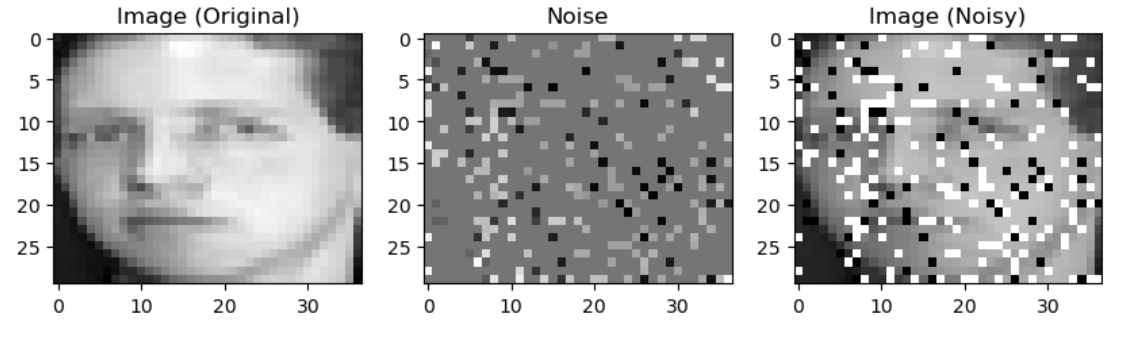
\includegraphics[width=0.85\textwidth]{figure/ORLnoise.png}
  \caption{Example of salt-and-pepper noise applied to an ORL face image.}
  \label{fig:ORLnoise}
\end{figure}
Figure~\ref{fig:ORLnoise} shows an example from the ORL dataset. The left image shows the original image, the middle image displays the added noise layer, and the right image presents the result after noise is added. It can be seen that black and white pixels are randomly distributed across the entire image, causing significant interference to the facial structure.
\begin{figure}[h]
  \centering
  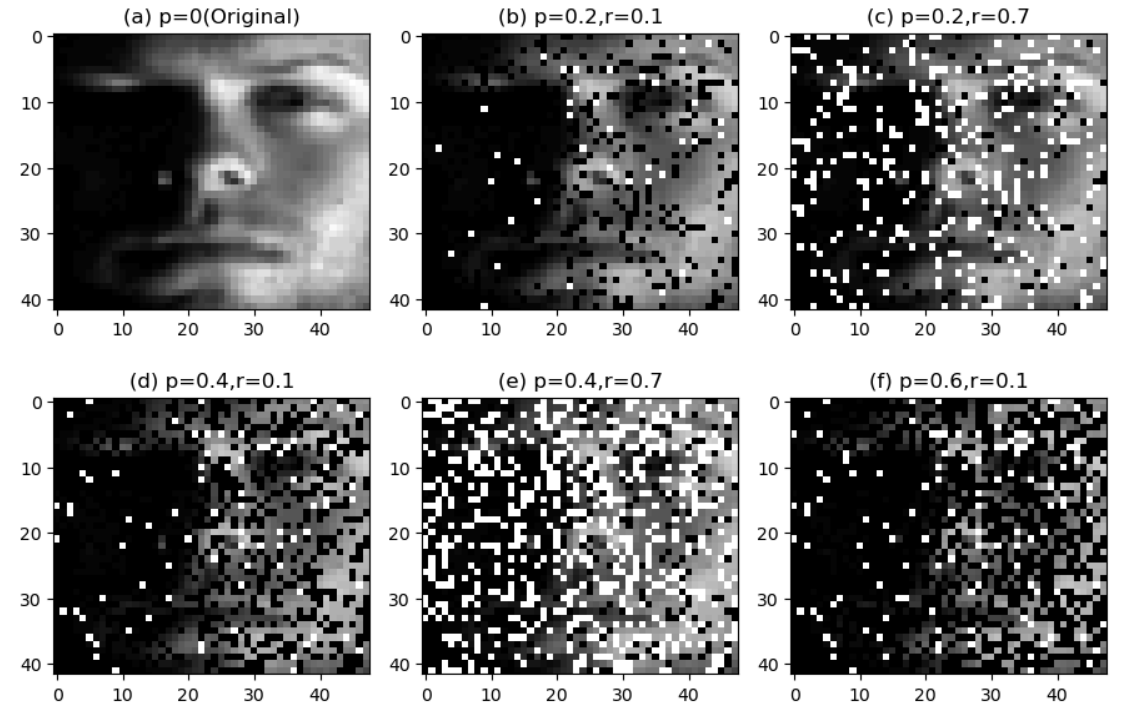
\includegraphics[width=0.9\textwidth]{figure/Yalebnoise.png}
  \caption{Examples of salt-and-pepper noise applied to the YaleB dataset under different parameter settings of $p$ and $r$.}
  \label{fig:Yalebnoise}
\end{figure}

Figure~\ref{fig:Yalebnoise} presents samples from the YaleB dataset under different noise settings. As the value of $p$ increases, the noise becomes denser and more destructive.  Adjusting the value of $r$ alters the ratio of black and white pixels, thereby changing the brightness distribution of the noise. These examples illustrate how salt and pepper noise impacts image appearance under various conditions, providing a basis for evaluating the robustness of the models we applied.

\section{Experiment}
In this study, two widely used face image datasets were employed: ORL and Extended YaleB. The ORL dataset contains 400 grayscale images from 40 subjects, with each subject having 10 photographs featuring different facial expressions and lighting conditions. The Extended YaleB dataset comprises 2,414 facial images of 38 subjects captured in 9 poses and 64 lighting conditions. To reduce computational complexity, the ORL images were resized from $92 \times 112$ to $30 \times 37$ pixels, while the YaleB images were resized from $168 \times 192$ to $42 \times 48$ pixels, and the pixel values were normalized to scale their range to [0, 1].

On the preprocessed data, we further added salt-and-pepper noise, controlling the noise level and proportion by adjusting the noise parameters $p$ and $r$. Two NMF algorithms were implemented for comparison: the standard $L_2$ NMF and $L_{2,1}$-Norm Based NMF, to evaluate their robustness under different noise conditions. The performance of each algorithm was evaluated using three metrics: Relative Reconstruction Error (RRE), Clustering Accuracy (ACC), and Normalized Mutual Information (NMI).


\subsection{Evaluation Metrics}
To comprehensively evaluate the performance of different NMF algorithms in noisy conditions, this experiment applies three common metrics: Relative Reconstruction Error (RRE), Clustering Accuracy (ACC), and Normalized Mutual Information (NMI). These three metrics evaluate model performance from different perspectives: RRE measures the algorithm's ability to reconstruct the original data, Accuracy reflects the classification consistency of decomposed features in clustering tasks, while NMI quantifies the amount of shared information between the clustering results and the true labels. The combination of these three metrics enables a comprehensive evaluation of the overall performance of the NMF algorithm in terms of reconstruction accuracy and clustering quality, providing a reliable basis for comparing the robustness of different algorithms\cite{sohrabi2025graph}\cite{hedjam2021nmf}.

\subsubsection{Relative Reconstruction Error (RRE)}
The Relative Reconstruction Error (RRE) is used to evaluate how well the reconstructed matrix $WH$ approximates the original clean data $\hat{X}$. It is defined as: 
\begin{align}
    RRE = \frac{\| \hat{X} - WH \|_F}{\| \hat{X} \|_F}
\end{align}
where $\hat{X}$ denotes the clean dataset, and $W$ and $H$ are the basis and coefficient matrices obtained from the NMF decomposition. The smaller the RRE value, the more accurately the algorithm reconstructs the original data, indicating superior stability and robustness. RRE is one of the fundamental metrics for evaluating NMF performance, providing an intuitive reflection of how different algorithms perform in reconstructing data under noisy conditions\cite{sohrabi2025graph}.

\subsubsection{Accuracy (ACC)}
The accuracy of clustering (ACC) is used to evaluate whether the features obtained from NMF decomposition can effectively preserve the class information of the original data. After decomposing $X = WH$, the coefficient matrix $W$ is regarded as the new feature representation. The K-means algorithm is then applied to the columns of $H$, where the number of clusters is set equal to the number of true classes. The accuracy is defined as:
\begin{align}
    Acc(Y, Y_{\text{pred}}) = \frac{1}{n} \sum_{i=1}^{n} \mathbf{1}(Y_{\text{pred}, i} = Y_i)
\end{align}
where $Y$ represents the true labels and $Y_{\text{pred}}$ denotes the predicted labels from clustering. The higher the ACC value, the better the low-dimensional features perform in preserving the class structure. Accuracy is a key metric for evaluating the performance of NMF-based algorithms, reflecting the ability of decomposed features to distinguish between different classes\cite{hedjam2021nmf}.

\subsubsection{Normalized Mutual Information (NMI)}
Normalized Mutual Information (NMI) is used to measure the consistency between the clustering results and the true labels. It evaluates the quality of clustering by calculating the mutual information between the two and normalizing it, defined as follows:
\begin{align}
    NMI(Y, Y_{\text{pred}}) = \frac{2 \times I(Y; Y_{\text{pred}})}{H(Y) + H(Y_{\text{pred}})}
\end{align}
where $I(\cdot)$ denotes the mutual information and $H(\cdot)$ represents the entropy. The NMI value ranges from 0 to 1, with higher values indicating that the clustering results are closer to the true classification structure. Compared to accuracy, NMI is not affected by the permutation of cluster labels and provides a more objective evaluation of clustering performance. NMI is often used in combination with ACC to comprehensively evaluate the performance of NMF algorithms in clustering tasks.

\subsection{Experimental results}

\subsubsection{Relative Reconstruction Error (RRE)}
Relative Reconstruction Error (RRE) is used to measure an algorithm's ability to reconstruct original images in noisy conditions. A smaller value indicates that the model can more accurately restore the original data and possesses greater robustness. In this experiment, we tested both $L_2$-NMF and L$_{2,1}$-NMF on the ORL and YaleB datasets with different combinations of noise parameters $p$ and $r$. The mean and standard deviation of RRE were calculated over multiple runs, and the results are shown in Figure~\ref{fig:RREORL} and Figure~\ref{fig:RRE YaleB}.
\begin{figure}[p]
    \centering
    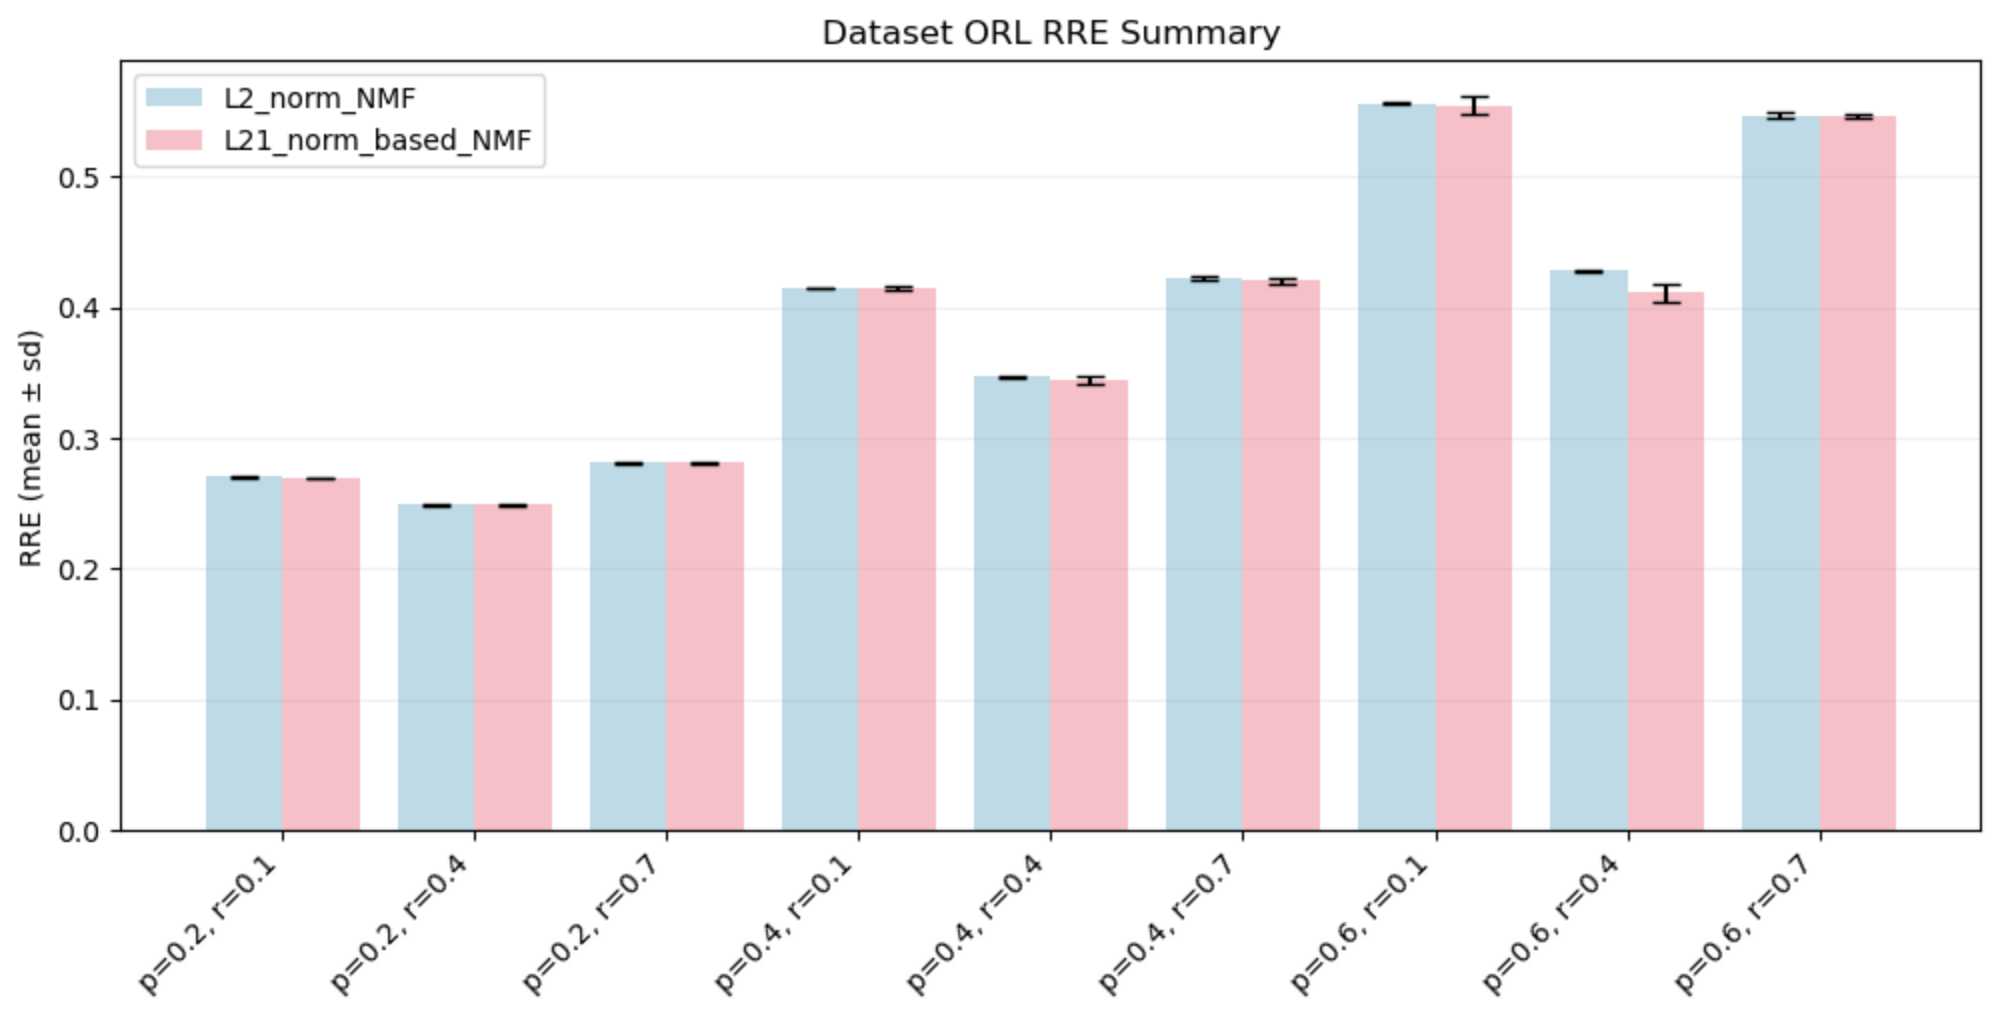
\includegraphics[width=0.9\linewidth]{figure/RRE ORL.png}
    \caption{Dataset ORL RRE Summary}
    \label{fig:RREORL}
\end{figure}

\begin{figure}[p]
    \centering
    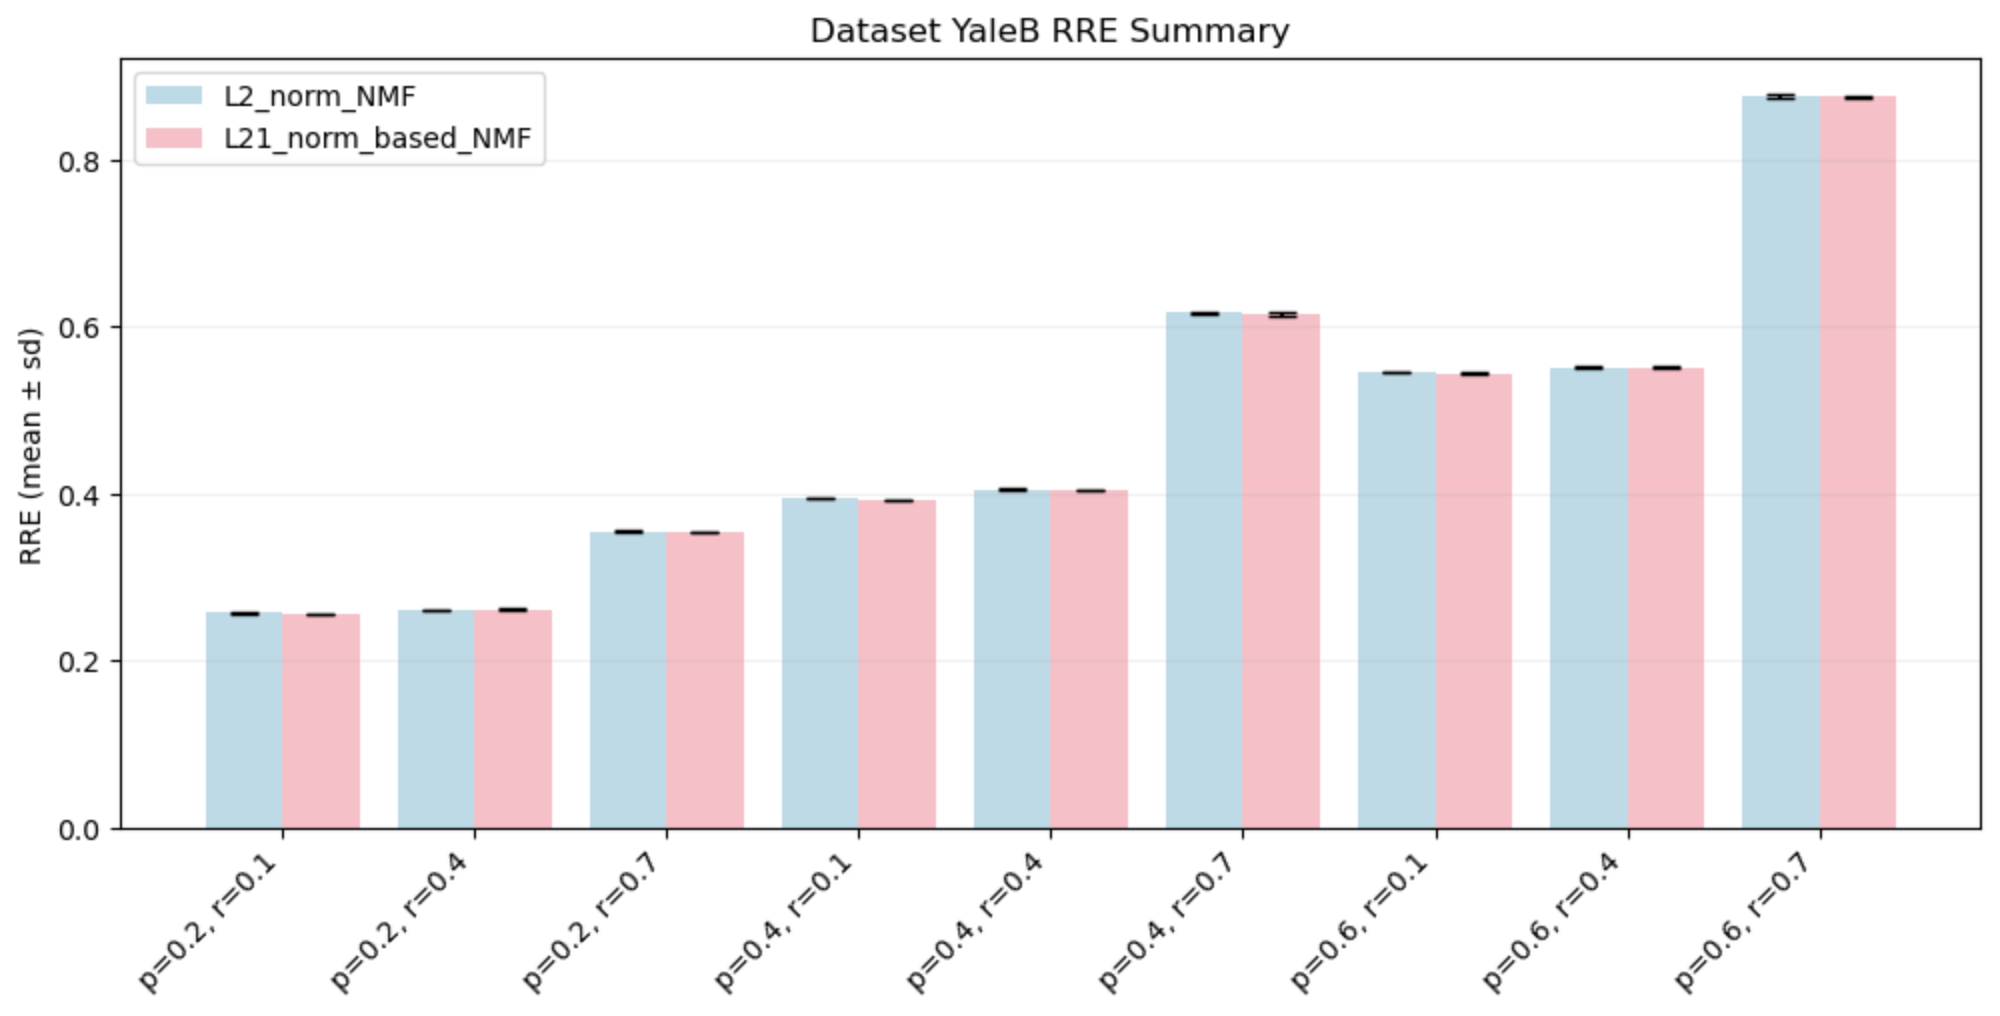
\includegraphics[width=0.9\linewidth]{figure/RRE YaleB.png}
    \caption{Dataset YaleB RRE Summary}
    \label{fig:RRE YaleB}
\end{figure}

The results show that as the noise level $p$ increases, the RRE values across all experiments exhibit a clear upward trend, indicating that higher noise levels significantly decrease the model's reconstruction accuracy. When the white noise proportion $r$ increases, the RRE also rises slightly, showing that white noise tends to have a stronger influence on image reconstruction.

Between the two algorithms, the overall performance is close, but the L$_{2,1}$-NMF shows slightly lower RRE values in most cases. For example, on the ORL dataset when $p=0.4$ and $r=0.4$, the RRE of $L_2$-NMF is 0.3471 while L$_{2,1}$-NMF is 0.3446. The gap becomes larger at higher noise levels, such as $p=0.6$. This result suggests that the L$_{2,1}$-NMF can deal with noisy pixels better and keep more stable reconstruction. The standard deviations are generally small, which means the results are stable and repeatable.

For the  datasets, the ORL dataset exhibits a lower overall RRE due to its smaller sample size and minimal facial conditions, withL$_{2,1}$-NMF having a more visible advantage. The YaleB dataset has more samples and complex lighting conditions, which makes its RRE values higher overall. However, under strong noise (for example $p=0.6$, $r=0.7$), the L$_{2,1}$-NMF still keeps slightly better reconstruction performance. 

In summary, L$_{2,1}$-NMF performs with stronger robustness under conditions of strong noise and non-Gaussian noise, consistent with its theoretical expectation. The detailed RRE results for all parameter settings can be found in Table~\ref{tab:orl_rre} and Table~\ref{tab:yaleb_rre} in the Appendix.

\subsubsection{Accuracy (ACC)}


To further evaluate the clustering performance of both algorithms, we calculated the clustering accuracy (ACC) under different noise settings $(p, r)$. Each experiment was repeated five times, and the mean and standard deviation were recorded.


The accuracy comparison results are shown in Figure~\ref{fig:orl_acc} and Figure~\ref{fig:yaleb_acc}.

\begin{figure}[p]
    \centering
    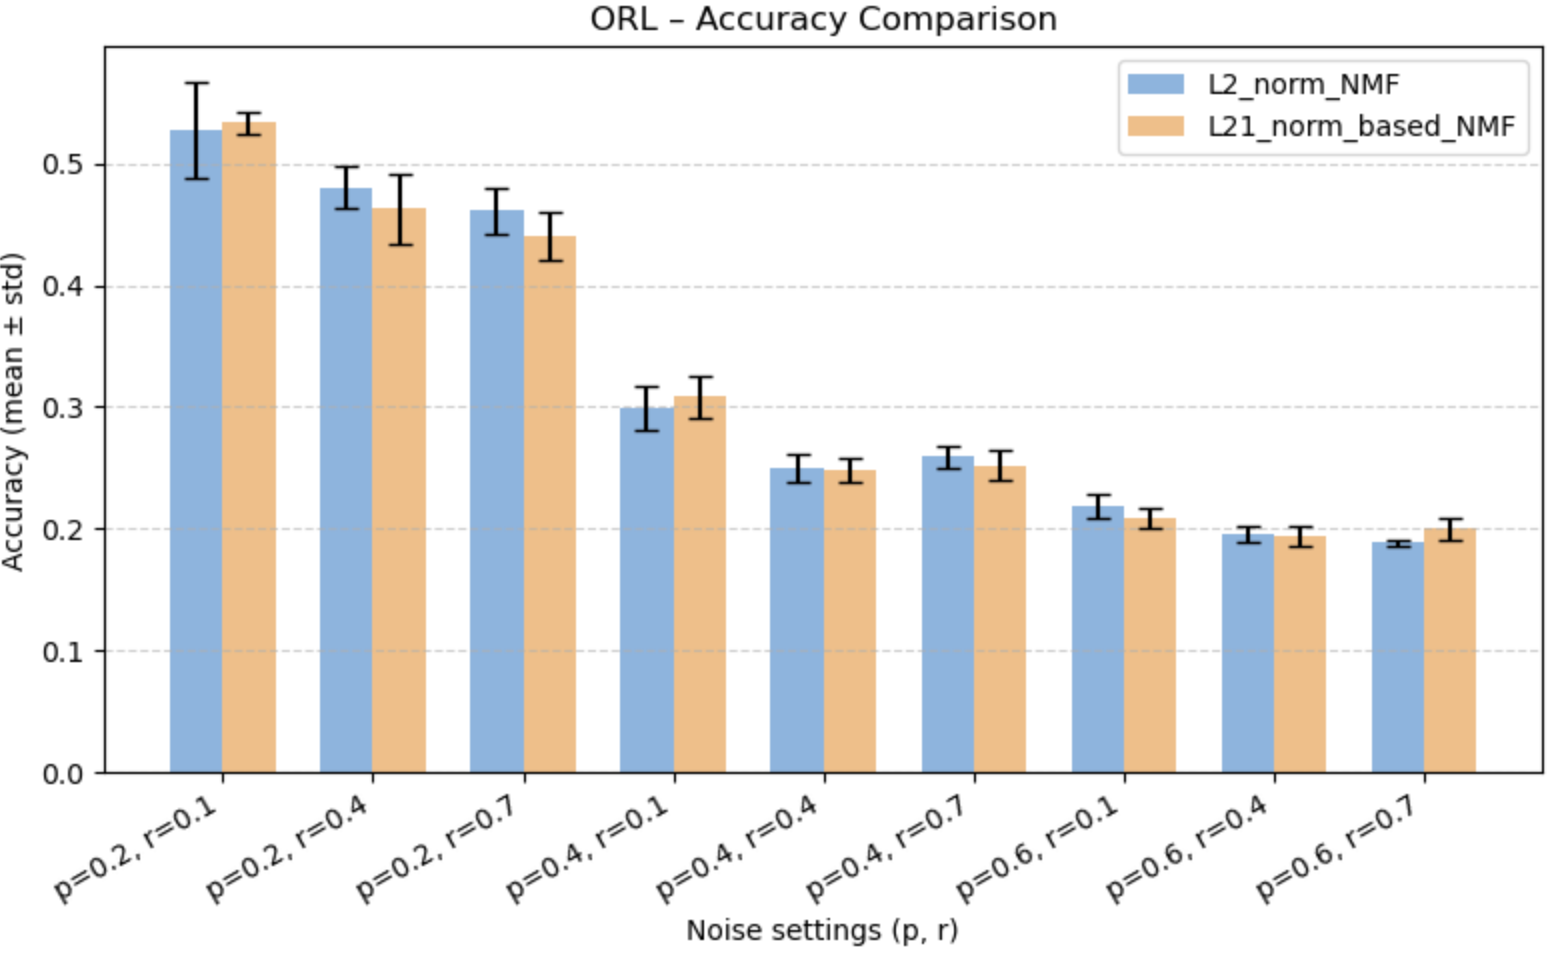
\includegraphics[width=0.9\linewidth]{figure/orl_acc.png}
    \caption{Dataset ORL ACC Summary}
    \label{fig:orl_acc}
\end{figure}

\begin{figure}[p]
    \centering
    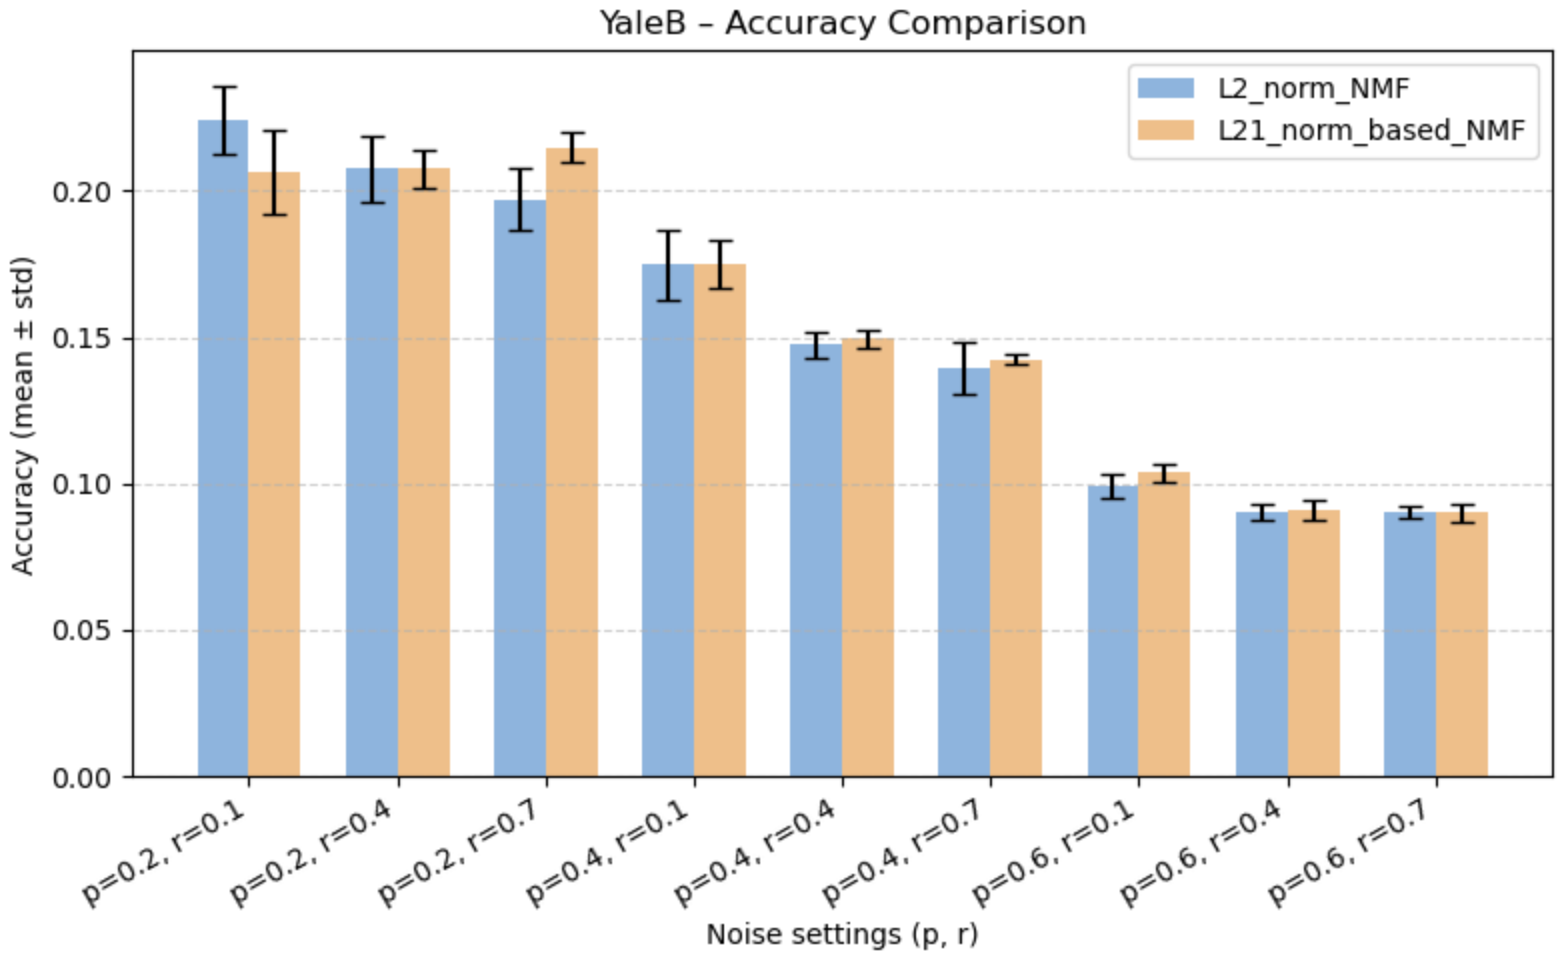
\includegraphics[width=0.9\linewidth]{figure/yaleb_acc.png}
    \caption{Dataset YaleB ACC Summary}
    \label{fig:yaleb_acc}
\end{figure}

The results indicate that as the noise level $p$ increases, the clustering accuracy of both datasets shows a significant downward trend. When $p=0.2, r=0.1$, the average accuracy on the ORL dataset is 0.5278 for $L_2$-NMF and 0.5339 for L$_{2,1}$-NMF. As the noise increases to $p=0.6, r=0.7$, the accuracy drops to 0.1883 and 0.2000 respectively. A similar pattern is observed in the YaleB dataset, where at $p=0.2, r=0.1$, the accuracies of $L_2$-NMF and L$_{2,1}$-NMF are 0.2242 and 0.2065, and they decrease to 0.0903 and 0.0901 when $p=0.6, r=0.7$.
This indicates that increased noise significantly weakens the model's ability to distinguish clusters in the clustering task.

When comparing the two algorithms, L$_{2,1}$-NMF achieves slightly higher accuracy in most cases. For example, on the ORL dataset at $p=0.4, r=0.1$, the accuracy of $L_2$-NMF is 0.2994, while L$_{2,1}$-NMF reaches 0.3083. Under high noise conditions ($p=0.6, r=0.4$), the accuracies are 0.1956 for $L_2$-NMF and 0.1933 for L$_{2,1}$-NMF. Although the difference in accuracy between the two algorithms is small, L$_{2,1}$-NMF is more stable in strong noise conditions and less sensitive to the influence of anomalous pixels.

For the datasets, the ORL dataset achieves higher overall accuracy than YaleB. This is mainly because ORL has fewer samples and minimal facial conditions and lighting conditions. In contrast, the YaleB dataset is significantly affected by lighting, making clustering more challenging and resulting in lower overall accuracy. Nevertheless, both algorithms show similar trends across the two datasets: accuracy decreases as noise increases, and L$_{2,1}$-NMF generally performs slightly better or comparably in most conditions.

The detailed numerical results are listed in Table~\ref{tab:orl_acc} and Table~\ref{tab:yaleb_acc} in the Appendix.

\subsubsection{Normalized Mutual Information (NMI)}
To further evaluate the clustering performance, we calculated the Normalized Mutual Information (NMI), which measures the consistency between clustering results and the true labels. Each experiment was repeated five times, and the mean and standard deviation were recorded. The comparison results are shown in Figure~\ref{fig:orl_nmi} and Figure~\ref{fig:yaleb_nmi}.

\begin{figure}[p]
    \centering
    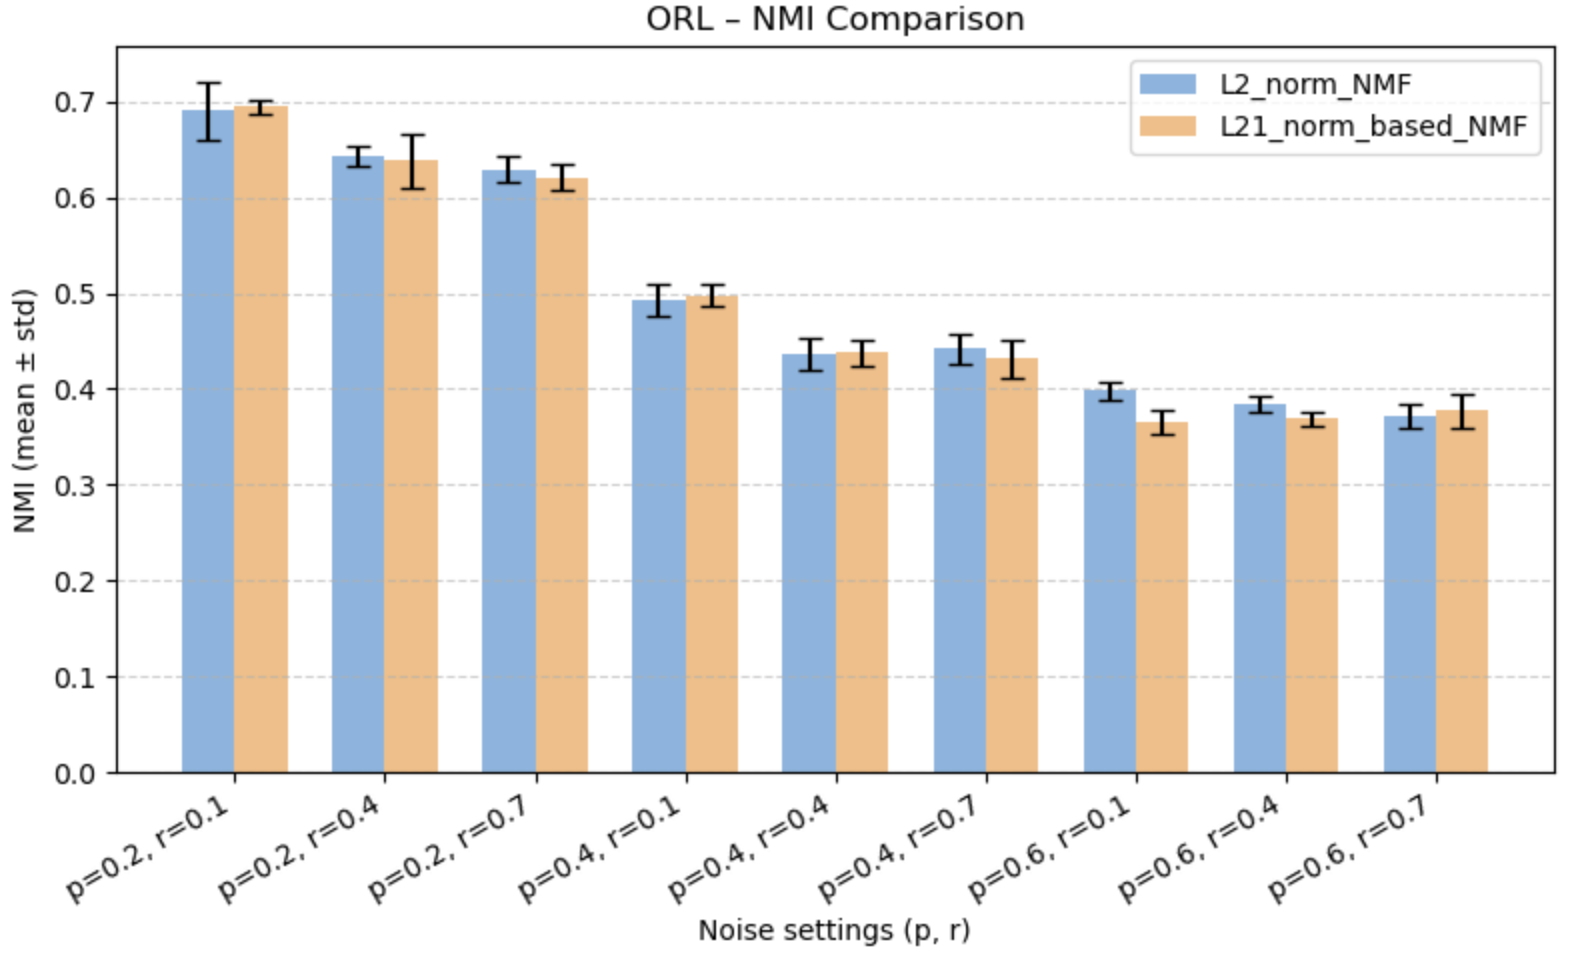
\includegraphics[width=0.9\linewidth]{figure/orl_nmi.png}
    \caption{Dataset ORL NMI Summary}
    \label{fig:orl_nmi}
\end{figure}

\begin{figure}[p]
    \centering
    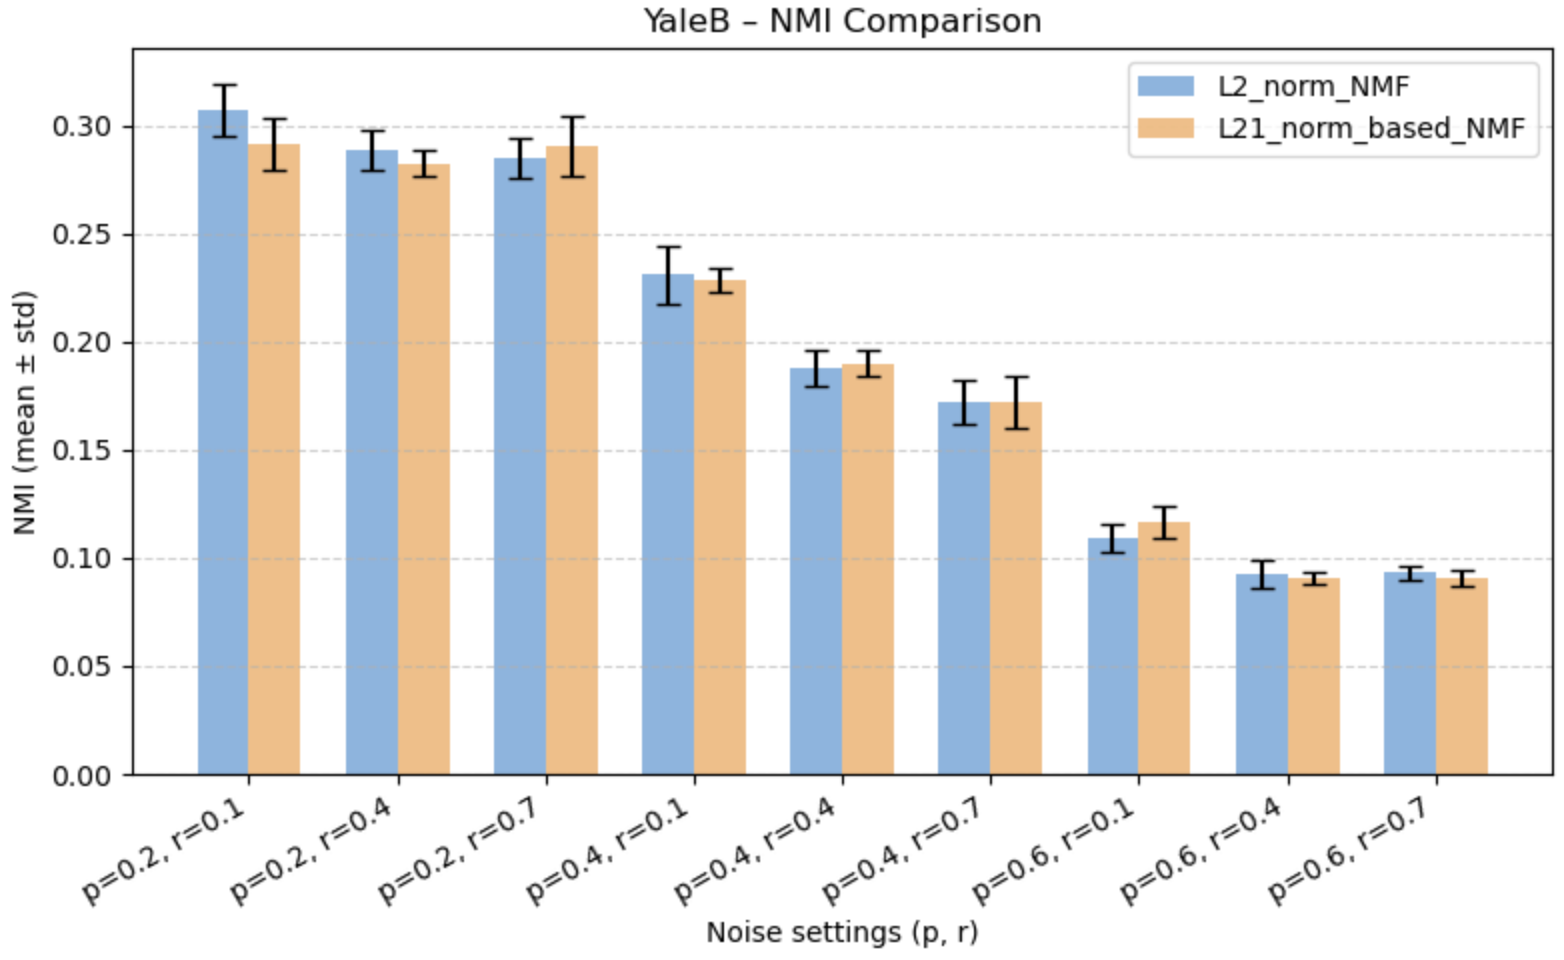
\includegraphics[width=0.9\linewidth]{figure/yaleb_nmi.png}
    \caption{Dataset YaleB NMI Summary}
    \label{fig:yaleb_nmi}
\end{figure}

As seen from the results, the NMI of both algorithms gradually decreases as the noise level $p$ increases. When $p=0.2, r=0.1$, the ORL dataset achieves an NMI of 0.6908 for $L_2$-NMF and 0.6948 for L$_{2,1}$-NMF. When the noise increases to $p=0.6, r=0.7$, the NMI drops to 0.3717 and 0.3769 respectively. A similar trend is observed on the YaleB dataset, where at $p=0.2, r=0.1$, the NMI is 0.3074 for $L_2$-NMF and 0.2910 for L$_{2,1}$-NMF, and decreases to 0.0931 and 0.0905 when $p=0.6, r=0.7$. It can be seen that higher noise levels weaken the correlation between the clustering results and the true labels.

In comparing the algorithms, the NMI value of L$_{2,1}$-NMF is slightly higher than that of $L_2$-NMF in most cases. Although the difference is not significant, it performs more stably in high-noise conditions. For example, on the ORL dataset at $p=0.4, r=0.4$, the NMI values are 0.4366 for $L_2$-NMF and 0.4376 for L$_{2,1}$-NMF; on the YaleB dataset at $p=0.4, r=0.1$, the values are 0.2308 and 0.2282 respectively. The differences are small but stable, indicating that L$_{2,1}$-NMF is more robust.

For the datasets, ORL has a higher overall NMI than YaleB, which is attributed to its smaller sample size and minimal facial conditions and lighting conditions. In contrast, YaleB's large sample size and complex lighting variations make it more challenging for models to preserve inter-class information structures. Overall, increased noise levels lead to a decline in NMI, but L$_{2,1}$-NMF maintains more stable clustering consistency under high noise.

The detailed numerical results are listed in Table~\ref{tab:orl_nmi} and Table~\ref{tab:yaleb_nmi} in the Appendix.

\section{Conclusion}
\subsection{Summary of work}

The main goal of this experiment is to study the robustness of different NMF methods in noisy environments. We used the $L_2$ NMF method and the $L_{2,1}$ norm based NMF method to study the performance of the datasets ORL and YaleB in the salt and pepper noise environment. We used the indicators Relative Reconstruction Error(RRE) and Accuracy/Normalized Mutual Information(Acc/NMI) to evaluate our results.

\subsection{Key findings}

From the experimental results, several trends are evident. 
First, both $L_2$ and $L_{2,1}$ NMF algorithms converge stably under all tested noise levels, but their performance differs across datasets and noise intensities. 
On the smaller ORL dataset, the $L_{2,1}$-norm NMF generally achieves lower reconstruction error (RRE) and slightly better clustering accuracy under low noise conditions, confirming its robustness to impulsive salt-and-pepper corruption. 
On the larger YaleB dataset, the two algorithms perform comparably in terms of RRE, while $L_{2,1}$ NMF shows slightly higher clustering accuracy when the noise ratio is moderate. 
As the noise proportion increases, both methods show clear degradation in accuracy and normalized mutual information (NMI), though $L_{2,1}$ tends to maintain more stable reconstruction performance. 
Overall, noise level has a strong and consistent impact on both algorithms, especially on the larger YaleB dataset.

\subsection{Interpretation and Insights}

The comparative results highlight complementary strengths of the two algorithms. 
The $L_{2,1}$-norm NMF demonstrates stronger robustness to sparse, high-intensity noise, as its row-sparse penalty suppresses the influence of corrupted samples, explaining its lower reconstruction errors on ORL. 
However, the $L_2$-norm NMF tends to preserve more global structure, which benefits clustering on large-scale datasets such as YaleB when the noise distribution is relatively uniform. 
These observations are consistent with previous findings \cite{Zeng2023RobustnessThreeNMF, Shen2022AdaptiveWeightedNMF, Liu2022RLNMF_AG}, indicating that robust NMF variants are advantageous under strong impulsive noise but not necessarily superior for clean or weakly corrupted data. 
In summary, $L_{2,1}$ is preferable when robustness is the main goal, whereas $L_2$ remains effective for large, structured datasets where noise is moderate and the focus is clustering performance.

\subsection{Limitations and Future Work}

We encountered many problems in our work, including:

\begin{itemize}
    \item The computational complexity is high, the operation time is long, and the convergence speed is slow.
    \item Few types of noise were tested. 
    \item The NMF method is highly sensitive to parameters.
\end{itemize}

\bigskip

We consider the following methods to improve the next step of the experiment:

\begin{itemize}
    \item Combined with the $L_1$ norm, a hybrid model is formed to evaluate its robustness.
    \item Introducing sparsity or graph regularization
    \item Use larger-scale or online updated NMF algorithms
\end{itemize}

\subsection{Closing Statement}

In summary, this paper verifies the robustness advantage of $L_{2,1}$ norm in non-negative matrix factorization through the study of $L_2$ NMF method and $L_{2,1}$ NMF method. The $L_{2,1}$ method can effectively maintain data structure and clustering performance in a high-noise environment. It provides a reliable theoretical and practical basis for real-world projects such as face recognition.
\pagebreak

\bibliography{bib.bib}
\bibliographystyle{ieeetr}

\pagebreak

\section*{Appendix}
\noindent \textbf{How to run the code?}

Our code needs to modify the local address of the data set at the beginning of the code to the root you need. \texttt{root\_ORL} refers to the root of ORL dataset. \texttt{root\_YaleB} refers to the root of YaleB dataset.

Then just run all code.

\begin{lstlisting}[language=Python]
root_ORL = 'data/ORL'
img_resize_ORL = (37,30)
root_YaleB = 'data/CroppedYaleB'
img_resize_YaleB = (48,42)
max_iter_nmf = 5000
max_iter_L21_nmf = 5000
\end{lstlisting}

\bigskip

\noindent\textbf{Contribution of each group member}

After group coordination, the three of us split the workload of coding and reporting roughly evenly, and in terms of group contribution, we each completed one-third of the total task.

\bigskip

\noindent\textbf{Results Summary}

\begin{table}[h]
\centering
\begin{tabular}{c c c c c c c}
\hline
\textbf{pr} & \textbf{L2} & \textbf{L2\_mean} & \textbf{L2\_std} & \textbf{L21} & \textbf{L21\_mean} & \textbf{L21\_std} \\
\hline
p=0.2, r=0.1 & L2 & 0.270295 & 0.000517 & L21 & 0.269087 & 0.000582 \\
p=0.2, r=0.4 & L2 & 0.248753 & 0.000753 & L21 & 0.248951 & 0.000938 \\
p=0.2, r=0.7 & L2 & 0.281011 & 0.000697 & L21 & 0.280894 & 0.000928 \\
p=0.4, r=0.1 & L2 & 0.414936 & 0.000245 & L21 & 0.414607 & 0.000931 \\
p=0.4, r=0.4 & L2 & 0.347132 & 0.000819 & L21 & 0.344625 & 0.002822 \\
p=0.4, r=0.7 & L2 & 0.421825 & 0.001625 & L21 & 0.420183 & 0.002430 \\
p=0.6, r=0.1 & L2 & 0.556032 & 0.000637 & L21 & 0.554477 & 0.006578 \\
p=0.6, r=0.4 & L2 & 0.427719 & 0.001062 & L21 & 0.410944 & 0.007375 \\
p=0.6, r=0.7 & L2 & 0.546857 & 0.001721 & L21 & 0.546262 & 0.001395 \\
\hline
\end{tabular}
\caption{Dataset "ORL" RRE Summary}
\label{tab:orl_rre}
\end{table}

\begin{table}[h]
\centering
\begin{tabular}{c c c c c c c}
\hline
\textbf{pr} & \textbf{L2} & \textbf{L2\_mean} & \textbf{L2\_std} & \textbf{L21} & \textbf{L21\_mean} & \textbf{L21\_std} \\
\hline
p=0.2, r=0.1 & L2 & 0.257389 & 0.000547 & L21 & 0.256240 & 0.000320 \\
p=0.2, r=0.4 & L2 & 0.261670 & 0.000199 & L21 & 0.261725 & 0.000645 \\
p=0.2, r=0.7 & L2 & 0.355032 & 0.000568 & L21 & 0.354162 & 0.000653 \\
p=0.4, r=0.1 & L2 & 0.394050 & 0.000305 & L21 & 0.392321 & 0.000620 \\
p=0.4, r=0.4 & L2 & 0.405109 & 0.000638 & L21 & 0.404892 & 0.000726 \\
p=0.4, r=0.7 & L2 & 0.616722 & 0.001437 & L21 & 0.615216 & 0.001507 \\
p=0.6, r=0.1 & L2 & 0.545179 & 0.000218 & L21 & 0.544295 & 0.000264 \\
p=0.6, r=0.4 & L2 & 0.551301 & 0.000974 & L21 & 0.551347 & 0.001026 \\
p=0.6, r=0.7 & L2 & 0.875648 & 0.002119 & L21 & 0.875193 & 0.002010 \\
\hline
\end{tabular}
\caption{Dataset "YaleB" RRE Summary}
\label{tab:yaleb_rre}
\end{table}

\begin{table}[p]
\centering
\begin{tabular}{c c c c c c c}
\hline
\textbf{pr} & \textbf{L2} & \textbf{L2\_mean} & \textbf{L2\_std} & \textbf{L21} & \textbf{L21\_mean} & \textbf{L21\_std} \\
\hline
p=0.2, r=0.1 & L2 & 0.5278 & 0.0398 & L21 & 0.5339 & 0.0092 \\
p=0.2, r=0.4 & L2 & 0.4806 & 0.0178 & L21 & 0.4628 & 0.0286 \\
p=0.2, r=0.7 & L2 & 0.4617 & 0.0189 & L21 & 0.4406 & 0.0195 \\
p=0.4, r=0.1 & L2 & 0.2994 & 0.0183 & L21 & 0.3083 & 0.0174 \\
p=0.4, r=0.4 & L2 & 0.2494 & 0.0116 & L21 & 0.2483 & 0.0092 \\
p=0.4, r=0.7 & L2 & 0.2594 & 0.0092 & L21 & 0.2522 & 0.0126 \\
p=0.6, r=0.1 & L2 & 0.2189 & 0.0095 & L21 & 0.2089 & 0.0087 \\
p=0.6, r=0.4 & L2 & 0.1956 & 0.0062 & L21 & 0.1933 & 0.0084 \\
p=0.6, r=0.7 & L2 & 0.1883 & 0.0021 & L21 & 0.2000 & 0.0088 \\
\hline
\end{tabular}
\caption{Dataset "ORL" Accuracy Summary}
\label{tab:orl_acc}
\end{table}

\begin{table}[p]
\centering
\begin{tabular}{c c c c c c c}
\hline
\textbf{pr} & \textbf{L2} & \textbf{L2\_mean} & \textbf{L2\_std} & \textbf{L21} & \textbf{L21\_mean} & \textbf{L21\_std} \\
\hline
p=0.2, r=0.1 & L2 & 0.2242 & 0.0119 & L21 & 0.2065 & 0.0145 \\
p=0.2, r=0.4 & L2 & 0.2076 & 0.0112 & L21 & 0.2077 & 0.0065 \\
p=0.2, r=0.7 & L2 & 0.1971 & 0.0107 & L21 & 0.2149 & 0.0053 \\
p=0.4, r=0.1 & L2 & 0.1748 & 0.0120 & L21 & 0.1750 & 0.0084 \\
p=0.4, r=0.4 & L2 & 0.1474 & 0.0045 & L21 & 0.1494 & 0.0030 \\
p=0.4, r=0.7 & L2 & 0.1394 & 0.0091 & L21 & 0.1425 & 0.0017 \\
p=0.6, r=0.1 & L2 & 0.0992 & 0.0044 & L21 & 0.1036 & 0.0033 \\
p=0.6, r=0.4 & L2 & 0.0904 & 0.0026 & L21 & 0.0907 & 0.0034 \\
p=0.6, r=0.7 & L2 & 0.0903 & 0.0020 & L21 & 0.0901 & 0.0030 \\
\hline
\end{tabular}
\caption{Dataset "YaleB" Accuracy Summary}
\label{tab:yaleb_acc}
\end{table}

\begin{table}[p]
\centering
\begin{tabular}{c c c c c c c}
\hline
\textbf{pr} & \textbf{L2} & \textbf{L2\_mean} & \textbf{L2\_std} & \textbf{L21} & \textbf{L21\_mean} & \textbf{L21\_std} \\
\hline
p=0.2, r=0.1 & L2 & 0.6908 & 0.0303 & L21 & 0.6948 & 0.0076 \\
p=0.2, r=0.4 & L2 & 0.6435 & 0.0104 & L21 & 0.6381 & 0.0289 \\
p=0.2, r=0.7 & L2 & 0.6294 & 0.0144 & L21 & 0.6202 & 0.0137 \\
p=0.4, r=0.1 & L2 & 0.4926 & 0.0159 & L21 & 0.4978 & 0.0120 \\
p=0.4, r=0.4 & L2 & 0.4366 & 0.0175 & L21 & 0.4376 & 0.0141 \\
p=0.4, r=0.7 & L2 & 0.4416 & 0.0152 & L21 & 0.4315 & 0.0205 \\
p=0.6, r=0.1 & L2 & 0.3986 & 0.0095 & L21 & 0.3661 & 0.0123 \\
p=0.6, r=0.4 & L2 & 0.3836 & 0.0080 & L21 & 0.3693 & 0.0075 \\
p=0.6, r=0.7 & L2 & 0.3717 & 0.0129 & L21 & 0.3769 & 0.0168 \\
\hline
\end{tabular}
\caption{Dataset "ORL" NMI Summary}
\label{tab:orl_nmi}
\end{table}

\begin{table}[p]
\centering
\begin{tabular}{c c c c c c c}
\hline
\textbf{pr} & \textbf{L2} & \textbf{L2\_mean} & \textbf{L2\_std} & \textbf{L21} & \textbf{L21\_mean} & \textbf{L21\_std} \\
\hline
p=0.2, r=0.1 & L2 & 0.3074 & 0.0120 & L21 & 0.2910 & 0.0120 \\
p=0.2, r=0.4 & L2 & 0.2885 & 0.0095 & L21 & 0.2824 & 0.0063 \\
p=0.2, r=0.7 & L2 & 0.2849 & 0.0092 & L21 & 0.2903 & 0.0139 \\
p=0.4, r=0.1 & L2 & 0.2308 & 0.0135 & L21 & 0.2282 & 0.0053 \\
p=0.4, r=0.4 & L2 & 0.1880 & 0.0085 & L21 & 0.1900 & 0.0062 \\
p=0.4, r=0.7 & L2 & 0.1721 & 0.0098 & L21 & 0.1718 & 0.0127 \\
p=0.6, r=0.1 & L2 & 0.1091 & 0.0068 & L21 & 0.1164 & 0.0074 \\
p=0.6, r=0.4 & L2 & 0.0921 & 0.0064 & L21 & 0.0909 & 0.0027 \\
p=0.6, r=0.7 & L2 & 0.0931 & 0.0031 & L21 & 0.0905 & 0.0036 \\
\hline
\end{tabular}
\caption{Dataset "YaleB" NMI Summary}
\label{tab:yaleb_nmi}
\end{table}






\end{document}
